\subsection{Loop Scheduling}
\label{sec:loopscheduling}

After the creation of the graph $G$ is complete, the scheduling step takes
place, scheduling independent operations in the most parallel way possible. In the 
best case there are no conflicting dependencies. For example in the calculation 
of the inner-product of two vectors (shown below) every operation is independent, 
as there are no data-dependency cycles, this is shown in the trasformation from
\figref{fig:innerproduct} to \figref{fig:innerproductmpcvec} in \secref{sec:mpcamortization}.
This independence means that, given the proper resources, every multiplication 
can be done in one step and vectorized into a temporary array. The summation of 
this temporary array is more complex, but only requires $\log_2N$ steps (again 
assuming adequate resources) in a manner similar to that shown
in \figref{fig:innerproductmpcvecdandc}. 
More commonly, dependent statements, especially across-loop dependencies, 
limit the amount of parallelization that can be done. The maximum parallelization 
between any two dependent statements depends on the $d$ value between those statements
that is calculated during the creation of the $G$ graph. 

The next phase is the actual scheduling algorithm. Recall that backward edges had
the negative weight $-1$ in all our examples, however, the weight on backward edges can be any value from $-1$ 
to $-(N-1)$. Forward edges have weight 0. Our algorithm proceeds in two phases: (1) strongly-connected component (SCC)
computation, and (2) scheduling. The first phase computes the strongly connected components in the graph $G$, intuitively,
each strongly connected component (SCC) consists of nodes that are interdependent and need to be scheduled accordingly. 
Once the SCC decomposition is done, we proceed to compute the schedule.



\subsubsection{SCC Decomposition}
\label{sec:SCC}

Consider a cycle $c \in G$. $d(c)$ is the absolute value of the sum of the weights of the edges in $c$. Consider a 
node $n \in G$. We say $n$ has \emph{constant rate} if all cycles $c$ through $n$ have the same $d(c)$. We write 
$d(n) = d(c)$. The $d(c)$ means that the computation at node $n$ at iteration $i$ depends on the computation 
at the same node $n$ at iteration $i-d(n)$. If $n$ is constant-rate with value $d(n)$, then for every $i$, $n(i)$
depends on the value computed at $n$ $d(n)$ iterations ago; but if the $d(c)$'s are not the same, then $n(i)$ depends on 
values computed at $n$ at different earlier iterations. This situation was illustrated earlier in~\figref{fig:fibconstantrate}. 

We extend the definition of constant-rate to $G$. We say that 
$G$ is constant-rate if all $n \in G$ are constant-rate. If $n$ is a node, such that there are no cycles through $n$ in $G$, 
then $d(n) = N$, or in other words, $n$ can be fully vectorized. If a node $n$ is not constant rate, we assign a default $d(n) = 1$ 
for the purpose of amortization. For the rest of the text, we are interested in constant-rate $G$'s and consider  
results on constant-rate $G$'s. In practice, nodes have $d(n)$ values of either $N$ or $1$ even though other values of 
$d(n)$ are possible in theory. We found that of the 23 loops we analyzed from the HYCC \cite{Buscher2018} 
benchmark suite none violated the assumption. A typical example is shown in \figref{fig:dbjoin2nonconstant}.
%only 1 did not follow our constant-rate assumption, this is shown in \figref{fig:dbjoin2nonconstant}. 
%\ana{TODO Ana: What are the implications of non-constant rate.}
% \ana{TODO Lindsey: can you show the example that is not constant rate?}
%\ana{Also, can you show here some stats on values of $d$ in those benchmarks? We don't have any values of d other than 1 or N, correct?}
%\ana{HERE HAVE TO GIVE empirical evidence, how good/bad it is.} \lindsey{does that work?}
\begin{figure}[h]
\centering
\begin{minipage}{0.7\textwidth}
\begin{javacode}
...
for(int i = 0; i < len; i++) {
    sum[i] = db[i*att+1] + db[i*att+2];
}
...
\end{javacode}
\end{minipage}
\caption{DB_JOIN2 from the HyCC benchmarks. There are no across-loop dependencies and the constant-rate assumption trivially holds.} 
\label{fig:dbjoin2nonconstant}
\end{figure}



%We will consider Strongly Connected Components (SCCs) in $G$. In the running example in~\figref{fig:MPCexample}(b), 
%we have two SCCs, $SCC_1$ consists of node 2, and $SCC_2$ consists of nodes $3,4,5$. 
Without loss of generality, we may assume that each cycle has the form $n_1 \rightarrow n_2 \rightarrow ... \rightarrow n_k \stackrel{-d}{\dasharrow} n_1$, 
or in other words, there is a single backward edge in the entire cycle. Even though cycles with $2$ or more backward 
edges are possible, such cycles can be transformed into $n$ disjoint cycles of the above form. The $-d$ on the
single backward edge in each of the $n$ cycles, is the sum of the $-d$'s of all backward edges in the original cycle. 
%\ana{TODO ANA: We probably need more here.}

\subsubsection{Amortized Schedule}
\label{sec:schedule}

We now compute the amortized schedule $\mathcal{A}$. 

%\lindsey{I am not sure what the figure fig:MPCexample is.... Ana, was that from the other paper? Or did I accedentally delete it or something?}

\begin{enumerate}


\item We begin by decomposing $G$ into Strongly Connected Components (SCCs). It is a theorem, that if $G$ is constant-rate, 
then for each $\mathit{SCC}$, and each pair of nodes $n_1, n_2 \in \mathit{SCC}, d(n_1) = d(n_2)$. We write $d(\mathit{SCC})$.
For the running example (code in~\figref{fig:ifthenelsedep} and graph $G$ shown in~\figref{fig:aikenscc}), we have two SCCs, 
$SCC_1$ consists of node 1, and $SCC_2$ consists of nodes $2,3,4$. $d(\mathit{SCC}_1) = N$ and $d(\mathit{SCC}_2) = 1$.

\item For each SCC, assume that there is a linear schedule $S: P_1 \rightarrow P_2 ... \rightarrow P_k$ given 
as input. $S$ takes into account only the forward edges in $G$: if $n_1, n_2 \in SCC$ and $n_1 \rightarrow n_2 \in G$, 
then $S(n_1)$ precedes $S(n_2)$ in the linear schedule. Note that computing an optimal schedule is NP-Hard, 
as we showed earlier, however, given a small SCC, one can brute force an optimal $S$. For the running example (graph $G$ shown in~\figref{fig:aikenscc}), 
we assume that nodes 2 and 3 perform the same operation. We work with schedule 
$S: \{2,3\} \rightarrow \{4\}$. It is important to note that with our treatment of arrays we have the same optimal schedule
for each iteration, as we have the exact same intra-loop dependences for each iteration.

%\ana{Also note, that due to our treatment of arrays we have the same schedule for each iteration of the loop, i.e., for each iteration, we either have a dependence edge or we don't.}

\item Given $S$ for a given SCC, we then compute the amortized schedule $\mathcal{A}({\mathit{SCC}})$; 
this is the schedule across all iterations of the loop for the given SCC. For each $P_i$ in $S$, there are $\lceil{\frac{N}{d(SCC)}}\rceil$
nodes in $\mathcal{A}_{\mathit{SCC}}$. $P_i(1),P_i(2),...P_i(d(SCC))$ go into node $P^1_i$, $P_i(d(SCC)+1),...P_i(2\cdot d(SCC))$ 
go into node $P^2_i$, etc. Recall that the parenthesized number denotes the iteration, e.g., $P_i(1)$ denotes $P_i$ at the first iteration 
of the loop. There are dependence edges as follows:
\begin{enumerate}
\item $P^j_i \rightarrow P^j_{i'}$ if there is an edge $P_i \rightarrow P_{i'}$ in $S$ (intra-loop edges).
\item $P^{\lceil{\frac{N}{d(SCC)}}\rceil}_i \rightarrow P^1_{i+1}$ for each $1 \le i < \lceil{\frac{N}{d(SCC)}}\rceil$ (across-loop edges).
\end{enumerate}
In the running example, $SCC_1$'s schedule is just the single vectorized node that executes all A's at once.
$SCC_2$'s schedule repeats $S: \{2,3\} \rightarrow \{4\}$ $N$ times: we have 
$\{2,3\}(1) \rightarrow \{4\}(1) \rightarrow \{2,3\}(2) \rightarrow \{4\}(2) ... \{2,3\}(N) \rightarrow \{4\}(N)$, 
as each iteration depends on the previous-iteration value computed at the same node.
This is illustrated graphically in~\figref{fig:unrolledloopdep}.   %\ana{Lindsey, can you draw this graph? It's basically just repeating A $->$ B,C $->$ B,C $->$ B,C etc.}

\item The decomposition of $G$ into SCCs gives rise to a DAG where the nodes in the DAG are the individual SCCs. 
If there is an intra-loop or an across-loop dependence edge from a node in $\mathit{SCC}_1$ to a node in $\mathit{SCC}_2$, 
then there is an edge from $\mathit{SCC}_1$ to $\mathit{SCC}_2$. The edges arise from intra-loop and from across-loop dependences, 
but note that across-loop dependences are rare, as they are typically accounted for within SCCs. We call this graph the SCC DAG.
The user gives a linearization of this DAG: $SCC_1 \rightarrow SCC_2 \rightarrow ... \rightarrow SCC_m$. 
The final schedule is as follows: $\mathcal{A} = \mathcal{A}({\mathit{SCC}_1}) \rightarrow \mathcal{A}({\mathit{SCC}_2}) ... \rightarrow \mathcal{A}({\mathit{SCC}_m})$.
In our running example, there is only one possible ordering of the two components, 
and the final schedule is as depicted in~\figref{fig:unrolledloopschedule}. %\ana{Lindsey, add the reference here to that figure you draw.}

%dependence edges $P(n)_1 \dasharrow P(n)_2 ... \dasharrow P(n)_{\lceil{\frac{N}{d(n)}}\rceil}$, reflecting the across-loop dependence 
%edges we saw earlier. The rest of the edges for every edge $n_1 \rightarrow n_2 \in G$ and every $1 \le i \le N$, add an edge 
%$G'(n_1(i)) \rightarrow G'(n_2(i))$ to $G'$ where $G'(n(i))$ returns the $P$ node in $G'$ that contains $n(i)$. 

\end{enumerate}

The test cases taken from the HyCC benchmark suite involved the manipulation of multi-dimentional arrays into output structures. 
This meant that almost all array accesses were independent - and those
that were dependent had simple constant rate dependencies. In addition most did not modify their own structure but were dependent 
on other arrays. None of the cases taken from the HyCC benchmark suite violated our assumptions 
this is further expanded on in \secref{sec:results}. 

%We assign a parallelization factor of $N$ to $n$, meaning that 
%$n$ can be fully vectorized. A more interesting case is a non-singleton $SCC$. Then there is at least one cycle 
%from $n$ to itself. We consider \emph{cycles} $c: n \rightsquigarrow n \in SCC$
%such that there is no repeated node in $c$, and sum up the edge weights along the edges in $c$. If all 
%cycles including $n$ have the same value $-d$, then we assign a parallelization factor of $d$ to $n$. That 
%means that $n$ depends on the value computed at $n$ exactly $d$ iterations earlier, and it does not depend 
%on node $n$ of iterations in-between. In contrast, if there are two distinct cycles with two different weights, 
%then we assign the default value of 1 to $n$. Intuitively, two distinct weights on cycles, say $-d_1$ and $-d_2$ 
%means that $n$ depends on the value computed at $n$ $d_1$ iterations ago and on the value computed 
%$d_2$ iterations ago. Taking all nodes in the SCC, if all nodes have the same parallelization factor $d$, 
%then we do nothing, otherwise we assign to all nodes factor -1. \ana{More intuition here, why is this important etc}

%\ana{Have to make some kind of claim that certain \% of bench falls under this assumptions or otherwise 
%our results don't count for much.} \lindsey{added}



\subsection{On the Correctness and Optimality of Schedules $\mathcal{A}$}
\label{sec:theoreticalguarentees}

In \secref{sec:mpcamortization} we stated our two main problems \problemref{problem:prob1}, to compute an optimal loop body schedule, 
and \problemref{problem:prob2}, to compute an optimal across-loop schedule. We note that the notion of optimality is restricted by the assumptions in
our model, outlined in \secref{sec:loopbodyanalysis}. Recall that we assume unlimited bandwidth as well as identical cost of execution, e.g.,
executing 1 MPC primitive costs 1, and executing 1000 primitives at once costs 1 as well. In our model, an optimal schedule is the shortest 
sequence of MPC primitives, some possibly vectorized, such that the sequence observes \emph{all} inter-loop and across-loop dependencies. 

\subsubsection{On Correctness of Schedules $\mathcal{A}$}

Problem 2 can be formulated on an unrolled loop as follows. 
Let $L$ be a loop body within an MPC program. %\ana{This needs to be revised. Take into account the MUX.} Due to the restrictions on MPC outlined in
As stated in \secref{sec:mpc} the loop bounds of $L$ are both \emph{static} and \emph{known at compile time}. 
$L$ can be unrolled while preserving program semantics. Each iteration is placed in line with
 the previous, and all variables of a specific iteration are renamed to be associated
only with that specific iteration. Dependencies between variables of different iterations can now be rewritten 
as dependencies between these newly renamed variables. Say, $L$ contains an 
across-loop dependency between variables $x$ and $y$ where $d$ is the number of iterations between 
the computation of $x$ and the computation of $y$. After unrolling the loop; the value of $x$ for 
iteration $i$ can be computed: $\forall i \in L, x_{i} = y_{i - d}$. This also holds for array 
accesses. 
%This creates a body of code that only executes once, the analysis of which
%is described in \problemref{problem:prob1}. 
Consider our running example in \figref{fig:arrayloop}. 
If we bound $i$ to 2 iterations we can unroll the loop and determine the dependencies, this is shown
in \figref{fig:flattenedloop}. This unrolling presents the \emph{sequential schedule} of the loop which we denote by  $\mathcal{S}$.
Importantly, the unrolling is done on the SSA-form of the loop body after scalar substitution. There are no MUX nodes
in our example, but in general there would be.
This sequential schedule $\mathcal{S}$ is the base line that we use to argue correctness
for the schedule our algorithm computes (after making use of the well-formedness property of arrays). 

%\lindsey{Ana, do you think that is too jarring?} \ana{Needs some work... So how are we distinguishing this.}\ana{This is great!}

\begin{figure}[h]
\centering
\begin{minipage}{0.7\textwidth}
\begin{javacode}
A1_1[1] = B0[1];              // A1 = update(A0,1,B0)
B1_1[1] = A1_1[1] * D0[0];    // B1 = update(B0,1,A1*D0)
C1_1[1] = A1_1[1] * D0[0];    // C1 = update(C0,1,A1*D0)
D1_1[1] = B1_1[1] * C1_1[1];  // D1 = update(D0,1,B1*C1)

A1_2[2] = B1_1[2];            // A1 = update(A1,2,B1)
B1_2[2] = A1_2[2] * D1_1[1]); // B1 = update(B1,2,A1*D1)
C1_2[2] = A1_2[2] * D1_1[1]); // C1 = update(C1,2,A1*D1)
D1_2[2] = B1_1[2] * C1_2[2]); // D1 = update(D1,2,B1*C1)
\end{javacode}
\end{minipage}
\caption{Unrolled loop of \figref{fig:arrayloop} with a static bound on the loop variable $1 \le i \le 2$. 
This is the sequential schedule $S$ for the example. After unrolling the across-loop def-use dependency 
between {\sf D[1] = ...} and {\sf B[2] = A[2] * D[1];} becomes explicit. We simplify the SSA of array variables 
slightly in order to avoid notational clutter.} 
%\ana{Lindsey, I think you can draw the dependence graph too? One part is the code and the other part is the graph.}
%\lindsey{Ana, did you not like this example?}\ana{I do!}
\label{fig:flattenedloop}
\end{figure}

Unfortunately, as we have stated, finding an optimal loop-body amortized schedule is NP-hard. 
Therefore, finding an optimal across-loop amortized schedule is NP-hard, just as is finding an optimal loop-body schedule.
However, we posit that loop bodies are typically small and therefore, it would be feasible to compute the shortest common 
supersequence using a brute force approach. It would not be feasible of course to use a brute force approach to compute
the shortest common supersequence for the sequential schedule.
Therefore, in our work we are interested whether certain regularity of across-loop dependencies and the availability of
an optimal loop-body schedule can lead to efficient computation of an optimal across-loop schedule.
%Our key premise is that one can an across-loop amortized schedule that always either improves
%or does not effect real-world loops the run time of real-world loops. Given certain properties of the loop, the amortized 
%schedule we compute in the previous section is always correct and can also be optimal depending on the
%nature of the SCC graph. 

The first theorem below establishes correctness, i.e., that $\mathcal{A}$ computes the same result as $\mathcal{S}$ where
$\mathcal{S}$ is the standard sequential schedule of the loop. The correctness result takes into account
the well-formedness conditions and parallelization using well-formed arrays.

\begin{theorem}(Correctness)
Let $\mathcal{A}$ be the amortized schedule (computed as in~\secref{sec:loopscheduling}) and let $\mathcal{S}$ be the standard sequential 
schedule of the loop. $\mathcal{A}$ preserves dependences, i.e., for every def-use chain $(d,u) \in \mathcal{S}$, we have that
$\mathcal{A}(d)$ precedes $\mathcal{A}(u)$ in $\mathcal{A}$ and there is no redefinition of $\mathit{LHS}(d)$ in any 
of the nodes from $\mathcal{A}(d)$ to $\mathcal{A}(u)$. (Here $\mathcal{A}(n)$ gives the node in the schedule that contains $n$).
\end{theorem}

\begin{proof} (Sketch)
The proof is by case analysis. Case 1 considers when the variable in the def-use 
chain is a scalar, and Case 2 considers when it is an array location. 
The key is to prove that if there is a def-use dependence in $\mathcal{S}$, then the same def-use dependence
is represented in $G$.
Case 1 is straightforward, as dependencies between scalar variables are handled in the standard way. 
For Case 2, there are again two cases, the first case is when the array is reduced to standard SSA, in which 
case case 2 reduces to case 1, and the second case when the array is well-formed under our well-formedness
conditions. 

Suppose we have an array write $d: \A[f(i)] = ...$ and an array read $u: ... = \A[f'(i)]$ that form a def-use relation, i.e., 
the location that is written at the array write is used at the array read. If the def and the use happen in the same 
iteration, say $k$, that means that $f(k) = f'(k)$ and therefore, $f(i) \cong f'(i)$. If there are other writes to the same
location, they would happen earlier in the iteration, and the writes $d': \A[f(i)]$ have been numbered accordingly so
that the latest one is $d$ and the only def-use link into $u$ is from $d$. Now suppose that $d$ happens in iteration $i$
and $u$ happens in iteration $i+d$. That means $f(i-d) = f'(i)$ and therefore $f(i-d) \cong f'(i)$ in the analysis. Again, 
without loss of generality we may assume that $d$ is the last write to that location in iteration $i$ and our analysis 
will add an appropriate dependence edge. There will be no other def-use link into $u$ because that would
violate the disjointness assumption. 

Since our schedule respects def-use links, it follows that $d$ is scheduled ahead of $u$. Since there is a unique def-use
link, it follows that there is no write into that location that may happen between the $d$ and the $u$. 
%\ana{TODO: Ana, more here!}
\end{proof}

Correctness of execution of $\mathcal{A}$ is a simple corollary of the theorem. This follows by induction. Assume that all statements that 
execute before a given statement $s$ in $\mathcal{A}$ compute the same result in $\mathcal{A}$ as in $\mathcal{S}$. We will consider 
the execution of $s$ and show that $s$ in $\mathcal{A}$ computes the same result as $s$ in $\mathcal{S}$. This is obvious from the 
theorem: the computation of the operands of $s$ precedes $s$ in $\mathcal{A}$ and by the inductive hypothesis, they compute the
same value as in $\mathcal{S}$; therefore, $s$ computes the same result. %\ana{TODO: Ana, more here.}

\subsubsection{On Optimality}

Unfortunately, optimality is more difficult to establish. Again, we stress that the notion of optimality is limited by our model. 
In the general case, computing an optimal across loop schedule will be NP-hard,
using the same argument as for the optimal loop-body schedule. We study different common schedules, and we claim that if the code
obeys our assumptions (well-formedness of arrays and constant-rate across-loop dependencies) typical schedules that arise in practice
will be optimal. We first prove that each SCC schedule, as computed by our analysis, is optimal. Then we consider a class of commonly occurring schedules
and we prove that the schedule $\mathcal{A}$ computed by our analysis is optimal. The classes of loops that we observed that exhibit optimal schedule
have a MapReduce-like structure --- there are one ore more map-like computations followed by a reduce-like computation. An example is Inner Product,
where point-wise multiplications can be vectorized, producing an array of products, and computing the sum amounts to a reduce of that array around 
the plus operation. In future work we plan to explore additional loops and build a larger and more comprehensive categorization of the classes
of loops that occur in practice.

%\lindsey{WES: call ut classes for which we can demonstrate optimality,
%Something like: We found that optimal scheudes occured mostly for simple SCCs....? not sure.} 
%Finally, we consider some preliminary results and conjectures for schedules of different shape.

\begin{lemma}(Optimality of SCC Schedules) Assuming an optimal schedule of the loop-body component of the SCC, well-formed arrays, 
and constant-rate $G$, then the $\mathcal{A}(SCC)$ computed in~\secref{sec:loopscheduling} is optimal.
\end{lemma}

\begin{proof} (Sketch)
Recall that the $\mathcal{A}(SCC)$ schedule has cost $n \cdot \lceil{\frac{N}{d(\mathit{SCC})}}\rceil$, where $n$ is the height (i.e., length) of the optimal 
schedule of the loop-body component. Since we have a strongly connected component and constant-rate across-loop dependencies, 
then for each pair of statements $s_1, s_2 \in SCC$ 
we have that $s_1$ in iteration $i+d$ depends on $s_2$ in iteration $i$, and vice versa,  $s_2$ in iteration $i+d$ depends on $s_1$ in iteration $i$.
Let $s_1$ be a statement in the first node in $\mathcal{A}(SCC)$, and let $s_2$ be a statement in the last node in $\mathcal{A}(SCC)$. 
Therefore we have
\[s_1 (1) \rightarrow ... \rightarrow s_2 (1) \dasharrow s_1(d+1) \rightarrow ... \rightarrow s_2 (d+1) \dasharrow ...\]
where the length of each solid arrow chain is optimal and of length $n$, and the length of the dashed arrow chain is $\lceil{\frac{N}{d(\mathit{SCC})}}\rceil$.
\end{proof}

%\ana{Need a sketch of proof}

The most common schedules involve a MapReduce-like pattern. All our running examples follow this pattern. The intra-loop dependence graph has the form $s_1 \rightarrow s_2 \rightarrow ... \rightarrow \mathit{SCC}_k \rightarrow s_{k+1} \rightarrow $. Here $s_1, s_2, ... s_{k-1}, s_{k+1},...$ give rise to special SCCs that can be fully vectorized. $s_1, s_2, ... s_{k-1}, s_{k+1}, ... $ can be fully vectorized, while $\mathit{SCC}_k$ can be scheduled optimally according to the $d(\mathit{SCC}_k)$. Intuitively, since all $s_1, s_2, ...s_{k-1}$ must execute before $\mathit{SCC}_k$, then ${k-1}$ is a lower bound on their execution. An additional constraint is that none of $s_1, s_2$, etc., can be executed in parallel with some of the iterations of $\mathit{SCC}_k$, in which case ${k-1} + \mathit{cost}(\mathit{SCC}_k)$ is a lower bound on the execution of $s_1 \rightarrow s_2 \rightarrow ... \rightarrow \mathit{SCC}_k$. 
This is formalized by the following theorem.

\begin{theorem}(Optimality of Common Schedules) Let the SCC DAG be a straight-line DAG: $\mathit{SCC}_1 \rightarrow \mathit{SCC}_2 \rightarrow ... \rightarrow \mathit{SCC}_k \rightarrow
... \rightarrow \mathit{SCC}_{n-1} \rightarrow \mathit{SCC}_n$ where $d(\mathit{SCC}_k) \le N$, while all other $d(\mathit{SCC})=N$. Let all dependence edges in the SCC DAG be triggered by intra-loop dependence edges, let there be intra-loop dependences from $s_{k-1}$ to every $s_k \in \mathit{SCC}_k$ and let there be intra-loop dependences from every $s_k \in \mathit{SCC}_k$ to $s_{k+1}$. The amortized schedule computed in~\secref{sec:loopscheduling} is optimal. %\ana{Still not done.}
\end{theorem}

\begin{proof} (Sketch)
The proof follows directly from the lemma. From the lemma, the schedule of $\mathcal{A}(\mathit{SCC}_k)$ is optimal. Since SCCs $1, 2, ...,k-1$ must be scheduled ahead of $\mathit{SCC}_k$
and none of them can be scheduled in parallel with an iteration of $\mathcal{A}(\mathit{SCC}_k)$. This is because there are intra-loop dependences from every $s_1, s_2, ... s_{k-1}$ to every $s_k$ in the $\mathit{SCC}_k$. Similarly, $s_{k+1},...$ must be scheduled after $\mathit{SCC}_k$ due to the corresponding intra-loop dependences. Therefore, the schedule we compute is an optimal schedule. 
\end{proof}

Even though we capture most common loop structures, and compute optimal schedules for those loop structures, we would like to relax our assumptions and produce optimality results for a larger class of loop structures. 
%Clearly the problem is NP-hard, however, structuring the loop into SCCs naturally partitions the loop into smaller components. We conjecture that computing optimal schedules for each SCC can be feasible due to the small size of the SCCs.  


%The principal problem when we have a SCC DAG where more than one of the SCCs are not fully vectorized, i.e., have we have some $d(\mathit{SCC}) < N$, is that different iterations can be scheduled in parallel, even in the restricted case when there are intra-loop dependences from every node in one SCC to every node in the other SCC. We consider the following problem and conjecture. 
%Consider two strongly connected components, each with $d=1$ and the following SCC DAG: $\mathit{SCC}_1 \rightarrow \mathit{SCC}_2$. 
%We compute a schedule as follows. Let the intra-loop graph of $\mathit{SCC}_1$ be $A$, and the intra-loop graph of the $\mathit{SCC}_2$ be $B$. 
%We compute the Shortest Common Supersequence of $A$ and $B$ denoted by $S = \mathit{SCS}(A,B)$. Let us partition $S$ into $A'S'B'$
%where $A'$ is the longest common prefix of $A$ and $S$ such that $S'B'$ is a supersequence of $B$. 

%Let $A'$ be the prefix and $B'$ be the suffix of $S$, 
%such that $A'$ is the longest common prefix of $S$ and of $A$, and $B'$ is the longest common suffix of $S$ and $B$. 
%If $A'$ or $B'$ is empty, then we compute the schedule by chaining $S$ $N$ times. Otherwise, we compute the Shortest Common Supersequence of $A'$ and $B'$
%and so on, appropriately chaining these supersequences to form a schedule. We conjecture that this algorithm yields an optimal schedule. \ana{Show this in the case when A' or B' is empty.}
%\ana{Needs work.}
%and consider A'' and B'' as before, and so on. If we chain the SCSs we get an optimal schedule.

%\ana{State conjecture. 2 SCCs with d = 1. We can compute an optimal schedule as follows. Compute the SCS of A and B. Let A' be the prefix and B' be the suffix, 
%such that A' is a common prefix of the SCS and of A, and B' is the longest common suffix of the SCS and of B. If A' or B' is empty, we are done, otherwise compute the SCS of A' and B'
%and consider A'' and B'' as before, and so on. If we chain the SCSs we get an optimal schedule.}

%\ana{TODO: Here opine on the differences between the vectorization problem and the problem in MPC.}

%\ana{Correctness theorem should come here...}

%\paragraph{Creating The SCC Schedule}
%\label{sec:sccschedulecreation}
%To create the amoritized schedule (the execution of SCC within G) we use the following steps. 
%Let $G$ be a constant-rate graph that entails a DAG $D$, where the nodes of $D$ are the strongly 
%connected components of $G$. If $D$ is linear, and each $SCC \in D$ entails a loop-body schedule 
%$S: P_1 \rightarrow P_2 ... P_k$ with a cost of $d$. The schedule is created by running each 
%$SCC \in D$ sequentially. Futhermore if $\nexists SCC_i \rightarrow SCC_j$, s.t. $d_i \neq d_j \land d_j \neq 1$
%then the schedule is optimal. If the above is \emph{not} true then an optimal scheule of the two 
%SCC nodes is not known (and possibly NP-Hard to discover) as it depends on which
%specific instructions within each SCC can be scheduled together. One can also use Aiken's result to compute an 
%optimal greedy schedule using $n^2$ iterations, where $n$ is the number of nodes 
%in the loop-body schedule \cite{Aiken1988}. \ana{Add citations.} \lindsey{is this just aiken? or does someone else also say this}

%\begin{theorem} (Optimal Conditions)
%Let $G$ be a constant-rate graph that entails a DAG $D$, where the nodes of $D$ are the strongly connected components of $G$. 
%If $D$ is linear, and each $SCC \in D$ entails a loop-body schedule $S: P_1 \rightarrow P_2 ... P_k$, s.t. (1) $S$ is optimal 
%and (2) for every $P_i, i<k$, for every $n_1 \in P_i, \exists n_2 \in P_{i+1}$, s.t. $n_1 \rightarrow n_2 \in G$, (3)
%$\nexists SCC_i \rightarrow SCC_j$, s.t. $d_i \neq d_j \land d_j \neq 1$ then $\mathcal{A}$ is optimal.
%\end{theorem}

%\begin{proof} (Sketch)
%This SCC schedule is optimal because 1) dependences are the same across the loop iterations, and 2) there is dependence between 
%iteration $i$ and iteration $i+1$, no node in $i+1$ can be computed before the last node, i.e., $P_k(i)$ has been computed, as all 
%nodes in $i+1$ depend on $P_k(i)$. Furthermore each SCC dependency $SCC_i \rightarrow SCC_j$ respects 
%$d_i = d_j \lor d_j = 1$ meaning there exists no schedule that will outperform linear execution. \lindsey{this last part seems wrong....}
%\end{proof}

\begin{figure}[H]
\centering
\begin{minipage}{0.50\textwidth}
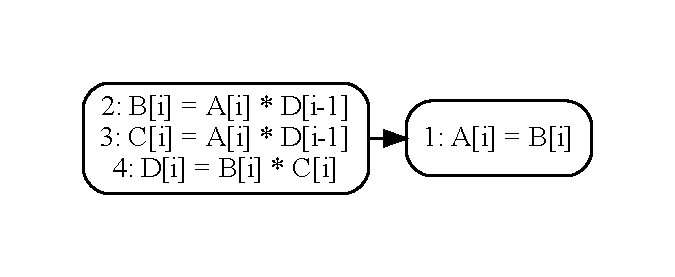
\includegraphics[width=\textwidth]{aikensccdag} 
\end{minipage}
\caption{SCC DAG for \figref{fig:arrayloop} formed from \figref{fig:aikenscc}.}
\label{fig:aikensccdag} 
\end{figure}

\subsubsection{Example} Consider our running example shown in \figref{fig:arrayloop}. There are three SCC nodes for this program. 
The first consists of line 1, while the second of lines 2 and 3, and the third line 4. This creates 
a DAG as shown in \figref{fig:aikensccdag}. The SCC node containing line 1 would be executed first 
with a $d$ value of 0 (assignments incur no cost). Next the node lines 2 and 3 are executed- both multiplications 
are performed at once incurring a cost and therefore $d$ of 1. The last node is also executed for a cost 
(and again a $d$ value) of 1. This is an optimal schedule for this exeuction as all of the 
$d$ values involved are only 1.

\subsection{Open Problems}

So far, we have identified a way of reasoning about loops as well as a way of computing schedules that turn out to be optimal 
for many loops in practice. Our work leaves a lot of open problems and future directions of research.

\paragraph{Optimality results} First, we believe that our results about optimality can be extended. A principal problem is, how do we schedule SCCs in the DAG that 
have $d$s different than $N$? The problem when we have a SCC DAG where more than one of the SCCs are not fully vectorized, i.e., we have some $d(\mathit{SCC}) < N$, is that different iterations can be scheduled in parallel, even in the restricted case when there are intra-loop dependences from every node in one SCC to every node in the other SCC.
We believe that we can compute optimal schedules per SCC and then combine those schedules to arrive at an optimal amortized schedule for the entire loop body.
%Even in the case when we have SCC1 connected to SCC2 via intra-loop edges, these two 
%SCCs can be scheduled in parallel as we can interleave the iteratio
%\ana{1. Extended proofs of optimality}

%\ana{2. Extension of results to nested loops}
\paragraph{Nested loops} Second, a further extension will be made for nested loops. The process begins at the innermost loop 
computing a vectorization, then inlining the vectorization within the enclosing loop.
Then the entire process can begin again.
%If there are no changes the variables that are in the outer loop dependecies  
%scheduling the nested loop this is trivial, as all input variables can be simply treated as constants. 
%However if any change does occur they must be reflected upon re-entering
%the outer loop, which may change the entire depedency. 
We leave this for future work.  %\lindsey{something like that, we should talk about it}.

%\ana{3. Divide and Conquer Parallelization}

\paragraph{Divide-and-conquer parallelization}
\label{sec:divideconquer}
% \lindsey{optomize certain operations that have a d value that does not equal 0. Do a divide and conquer}
Once the $d$ values are determined there are in general a lot of SCCs with $d=1$. 
%and all operations with $d = 0$ are fully amortized the next step is 
%to vectorized the remaining operations. 
Following the dependences as we did so far yields that full vectorization is not possible. For example, 
the sum in the Inner Product example will be $O(N)$. However, a divide and conquer 
algorithm can still reduce the overall running time when the aggregation operation has certain properties. 
For example consider (c) in \figref{fig:innerproduct}.
It is easy to see that the $d = 1$ in the addition on line 6, \texttt{sum} is dependent on its own previous value. 
If computed in the way shown, obeying all intra-loop and across-loop dependences, it will take $N$ steps, where $N = \vert C \vert$. 
This can be greatly reduced using a divide and conquer method, which is possible because the addition is an associative
operation. Consider the code in \figref{fig:innerproductmpcvecdandc}.
this shows how the number of operations in inner product can be reduce to $1 + \log_2 N$ steps. %More formally 
%this is shown in \lemref{lem:vecotrizationlemma}. 
By using this technique dependent operations can be computed
faster reducing the overall run time of the vectorized program. We plan to explore this direction in future work.
The principal problem is proving associativity of the loop computation.

%\begin{lemma}
%Given an vector $V$ and an associative operation $O$ with $K$ operands all
%operations can be completed in $O(log_K \vert V \vert)$ time.
%\label{lem:vecotrizationlemma}
%\end{lemma}




% 1. Add an edge from the conditional node, Cond, to the corresponding MUX node. This is just a forward edge.

% 2. Constructing the ``forward'' portion of the graph. If V is a scalar, add a forward edge $n_1 \rightarrow n_2$ such that for some $V_k$,
% $V_k \in LHS(n_1)$ and $V_k \in RHS(n_2)$. For arrays, add a forward edge $n_1 \rightarrow n_2$ such that there is $A_k[f(i)] \in LHS(n_1)$ 
% and $A_k[f'(i)] \in RHS(n_2)$ and $f(i)$ and $f'(i)$ are "equivalent", i.e., the same for all i. (Usually these equivalent accesses are just
% A[i]).

% 3. Constructing the "backward" portion of the graph. For each scalar $V$, let $n_1$ be the node such that $V_\mathit{max} \in LHS(n_1)$,
% i.e., this is the node that defines the $V$ exposed at the exit of the loop. Add an edge $n_1 \stackrel{-1}{\dasharrow} n_2$
% for each $n_2$ such that $V_0 \in RHS(n_2)$. In other words, $n_2$ has an upward exposed use of $V$, i.e., one that comes
% from. For each array write, let $n_1$ be the node such that $A[f(i)]_\mathit{max} \in LHS(n_1)$. Add an edge
% $n_1 \stackrel{-d}{\dasharrow} n_2$ for each $n_2$ such that $A_0[f'(i)] \in RHS(n_2)$ and $f(i-d) \cong f'(i)$.
